\documentclass[conference]{IEEEtran}
\IEEEoverridecommandlockouts
% The preceding line is only needed to identify funding in the first footnote. If that is unneeded, please comment it out.
\usepackage{cite}
\usepackage{amsmath,amssymb,amsfonts}
\usepackage{algorithmic}
\usepackage{graphicx}
\usepackage{textcomp}
\usepackage{xcolor}
\usepackage{hyperref}
\def\BibTeX{{\rm B\kern-.05em{\sc i\kern-.025em b}\kern-.08em
    T\kern-.1667em\lower.7ex\hbox{E}\kern-.125emX}}
\begin{document}

\title{COMP5048 Assignment 2 (Group)}

\author{\IEEEauthorblockN{Sasha Jenner}
\IEEEauthorblockA{490390494}
\and
\IEEEauthorblockN{Sebastian Kobler}
\IEEEauthorblockA{480377661}
\and
\IEEEauthorblockN{Minerva Predavec}
\IEEEauthorblockA{490398308}
\and
\IEEEauthorblockN{Xingyu Wei}
\IEEEauthorblockA{510585831}
\and
\IEEEauthorblockN{Huayue Zhang}
\IEEEauthorblockA{520196900}
}

\maketitle

\begin{abstract}
Over the past few decades, many different kinds of mobile devices have emerged. Some new mobile devices have succeeded in capturing the market, but some have failed. The best-selling type of mobile device has also varied over time, and not always has one device been dominant in the market. In this assignment, we used multiple interactive visualisations to explore what the mobile devices market looks like and how it has changed between 1989 and 2013.
\end{abstract}

\begin{IEEEkeywords}
mobile devices, visualisations
\end{IEEEkeywords}

\section{Mobile Device Types}
\label{sec:A}
%What types of mobile devices have been introduced between 1989 and 2013? Can you visually find common characteristics/features to define types of mobile devices?

There are six types of mobile devices which have been introduced between 1989
and 2013:
\begin{enumerate}
	\item smartphones,
	\item dumbphones,
	\item personal digital assistants (PDAs),
	\item palmtops,
	\item satnavs and
	\item tablets.
\end{enumerate}

Let the aspect ratio $r$ be the ratio of length to width given by
\[ r = \frac{\text{length}}{\text{width}}. \]

The implications of this are portrait mobile devices such as phones will
have $r>1$ and landscape mobile devices such as palmtops will have $0<r<1$.
%This will become a useful metric for differentiating between mobile device types.

Smartphones and dumbphones are both mobile telephones but are differentiated by
their computational abilities. Smartphones have an extensive operating system
which enables internet access, gaming, video and image photography. Dumbphones,
on the other hand, are not as extensive and are powered by less advanced
hardware. These are typically portrait hand-held devices with $r>1$.

PDAs were mobile devices which functioned as personal information managers. They
were usually portrait devices with touch screen and internet functionality.
However, since the advent of the smartphone these devices have mostly been
displaced.

Palmtops, tablets and satnavs are (usually) all landscape mobile devices with $0<r<1$.
Palmtops are miniature laptops which fit into ones palm or pocket. Historically,
palmtops were commercially popular during the late 1990s to early 2000s
\cite{palm}.
Tablets on the other hand are relatively large smartphones which were
popularised by the 2010 release of the first Apple iPad \cite{ipad}.
Satnavs, or satellite navigation devices, help users to navigate by pinpointing
their location using global navigation satellite systems (GNSS).

We will now investigate the defining characteristics of these mobile
devices types as is observed in the data.

\subsection{Visualisation} \label{sec:Avisu}
%Interactive Visualization (or multiple visualizations) allows you to “see” the pieces of information that lead to the answers to the above three questions 1-A/B/C.

A screenshot of an interactive scatter plot of length against width for all
mobile devices in the data, coloured by release year, is shown in Figure
\ref{fig:length-width-cyear-shot}. The diagonal divides the plot into two
classes; the portrait devices above the diagonal and the landscape devices
below the diagonal.
Through interaction, the portrait devices were understood
to be phones or PDAs and the landscape devices; palmtops, satnavs or tablets.

\begin{figure}
    \centering
    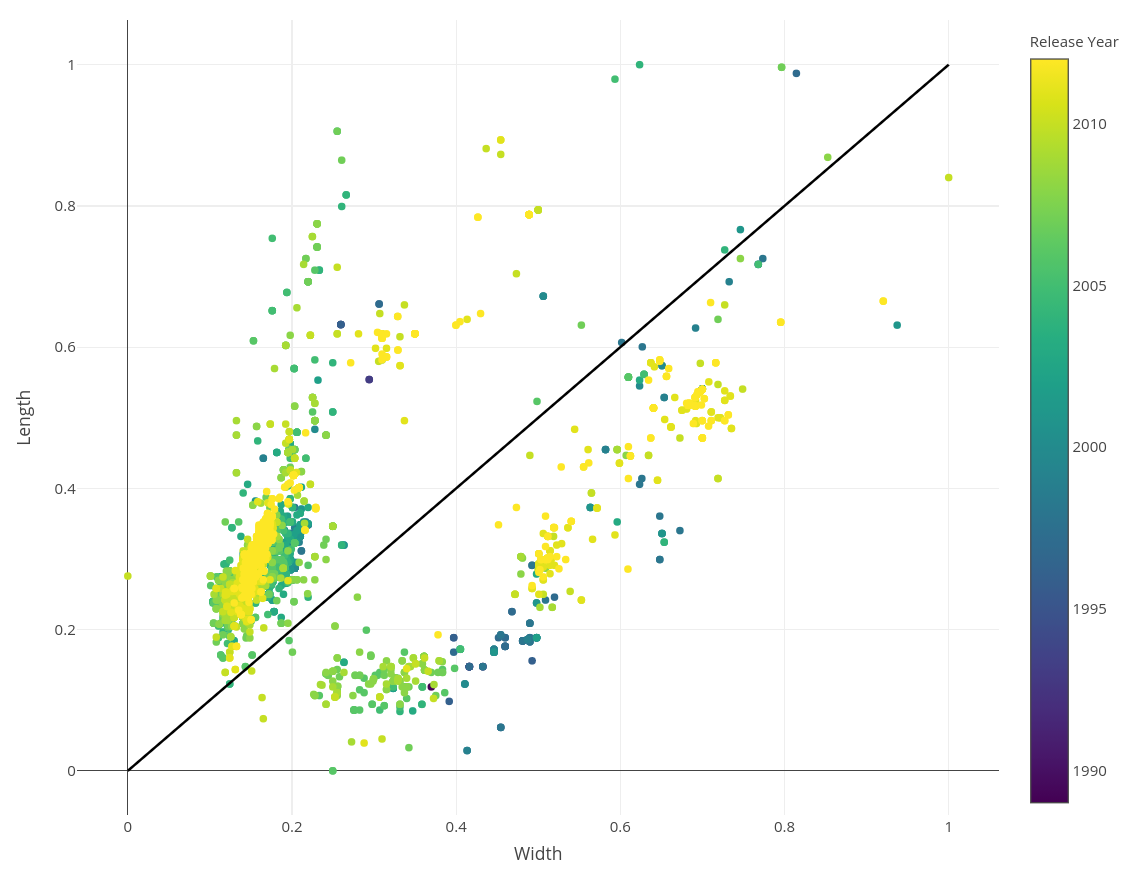
\includegraphics[width=0.5\textwidth]{../Visualisations/A/length-width-cyear-shot.png}
	\caption{\label{fig:length-width-cyear-shot}A screenshot of an
	interactive scatter plot displaying length against width for all the
	mobile devices in the data, coloured by their release year. The diagonal
	represents all square mobile devices with $r=1$. Those mobile devices
	above the diagonal are portrait devices with $r>1$, and those below the
	diagonal are landscape devices with $0<r<1$. Note that the axes do not
	have units since they have been normalised.}
\end{figure}

To understand the class of portrait devices, Figure \ref{fig:ddiag-diag-ccpu-shot}
was created, which plots the display diagonal against the diagonal of all
devices with $r>1$, coloured by CPU clock speed.
%It was discovered that display diagonal is proportional to CPU clock speed
%which makes sense.
Mobile devices in the top left area are fast with large displays
which contribute to most of their size. Whilst those in the bottom right area
have smaller displays, many functional buttons such as a keypad and less CPU
power. The bottom left area usually accounted for flip phones. Naturally, this
allowed us to differentiate the portrait mobile devices into smartphones,
dumbphones and PDAs.

%There are two distinct classes of phones, those with a screen that takes up most of their size, and those that have smaller screens to allow for keypads. These are respectively termed smartphones and dumbphones. However, a lot of the phones that were classified as smartphones actually turned out to be PDAs. Since true smartphones weren't introduced until 2007, this was picked as a dividing point, even though the transition was not sharp.

\begin{figure}
    \centering
    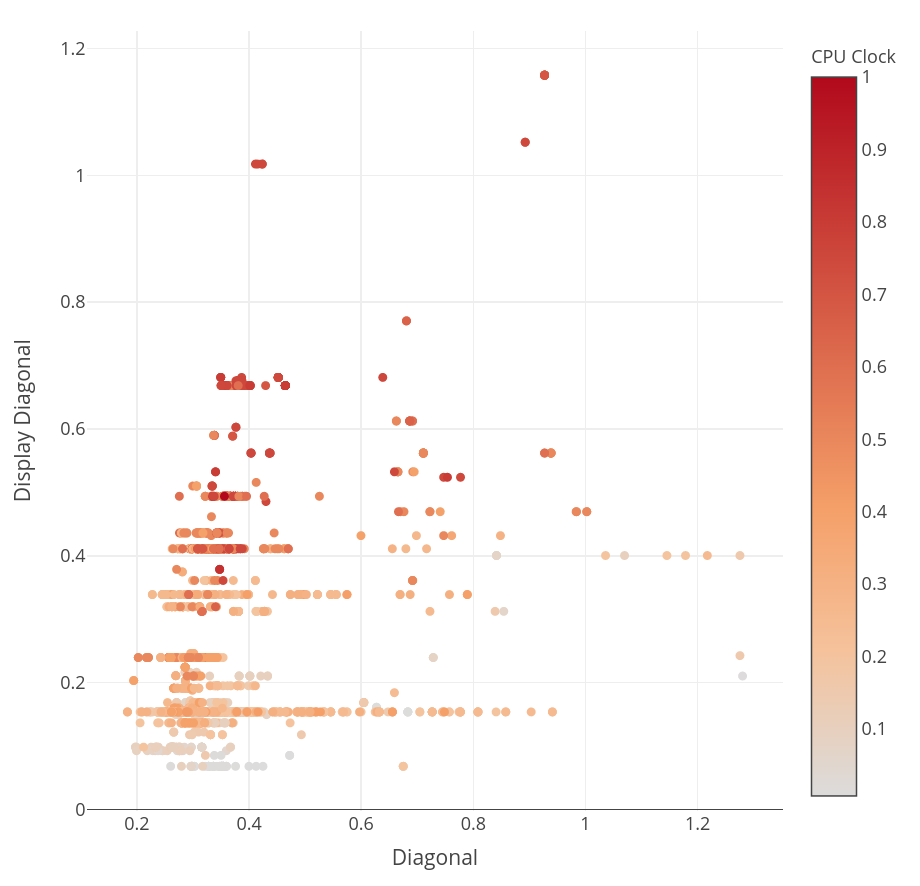
\includegraphics[width=0.5\textwidth]{../Visualisations/A/ddiag-diag-ccpu-shot.png}
	\caption{\label{fig:ddiag-diag-ccpu-shot}A screenshot of an interactive
	scatter plot showing display diagonal against diagonal
	for all the portrait devices in the data (with $r>1$), coloured by their
	CPU clock speed (normalised). Both diagonals are calculated by using
	Pythagoras' formula given the normalised overall and display length and
	width.}
\end{figure}

Now we will investigate the class of landscape devices. Consider again Figure
\ref{fig:length-width-cyear-shot} and the region below the $r=1$ diagonal. It
was found, through hovering over the model description of each point, that
devices with a width less than 0.4 in the green cluster mostly consist of
satnavs. Devices with a width greater than 0.4 and released before 2001
(coloured purple to blue) were found to be palmtops and the remainder
(coloured green to yellow) as tablets.

%The distinction between palmtops and laptops can be determined by the width - below a certain size, they are called palmtops due to the fact they can fit in a palm. Tablets are classified in the same way as laptops, except they are divided by date in a similar manner to PDAs.

Based on these observations, Figure \ref{fig:HeightvsWidth} shows the length
against width of all mobile devices coloured by their estimated type.
%Figure \ref{fig:HeightvsWidth} plots device width against device length.
%Figure \ref{fig:DevicevsDisplay} plots the device aspect ratio against the display aspect ratio.
%Each device is assigned a unique colour so the clusters in the data are easily visualised.
%Insert the single visulisations with the colours - both for the width and height, and the aspect ratios

\begin{figure}
    \centering
    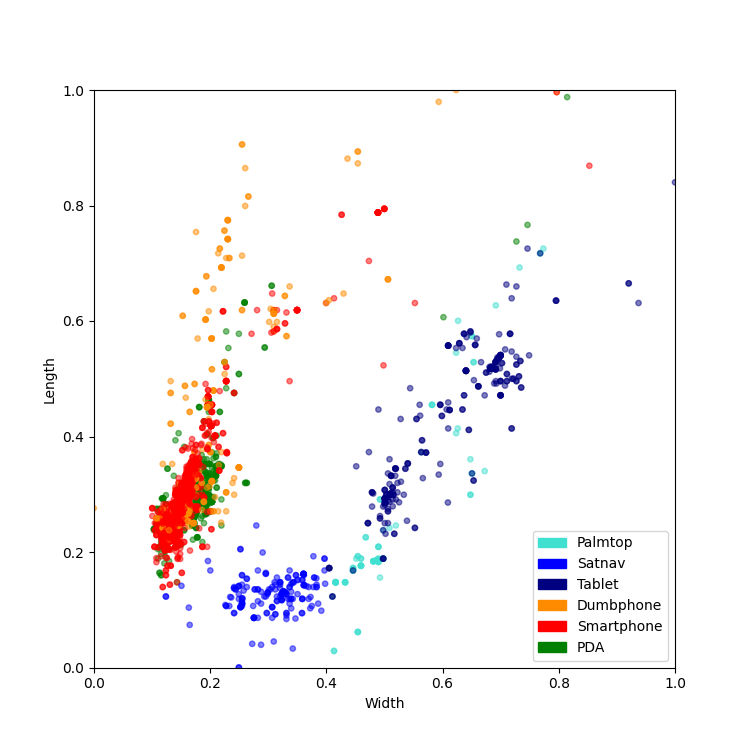
\includegraphics[width=0.5\textwidth]{../Visualisations/A/length-width-ctype.png}
    \caption{Length against width for all the mobile devices in the data,
	coloured by their estimated type. Note that the axes do not have units
	since they have been normalised.}
    \label{fig:HeightvsWidth}
\end{figure}

%\begin{figure}
%    \centering
%    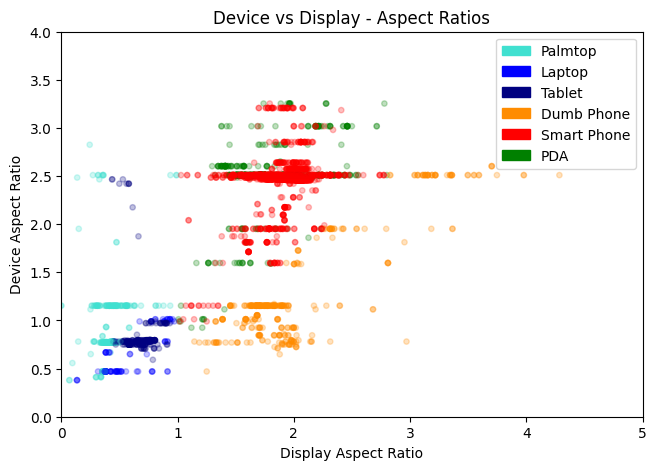
\includegraphics[width=0.5\textwidth]{../Visualisations/A/DevicevsDisplayColour.png}
%    \caption{}
%    \label{fig:DevicevsDisplay}
%\end{figure}

\subsection{Design Evaluation}
%Explain how your interactive visualisation has been evaluated and what sort of changes/modifications were applied to derive your final interactive visualisation.

%Exploratory data analysis of comparing different aspects against each other was used to find these initial types.
%Once the types were discovered, colours were added, and the two visualisations that mostly clearly illustrated the characteristics that defined them were created. It was found that the best axis assignments to separate the mobile devices into their respective types was length vs width as well as device vs display aspect ratios. This makes sense as often times we define these device types by their sizes, an example being comparing a tablet to a smartphone, whereby the tablet is clearly larger in both dimensions.

The interactive visualisations were evaluated on their utility, comprehension
and insightfulness. These were judged respectively by how well the visualisation
was to use, understand and make new insights from.

One modification made as a result of such evaluation was the $r=1$ line in
Figure \ref{fig:length-width-cyear-shot}, which was included after users
found it difficult to locate the distinction between portrait and landscape
devices. Similarly, colouring by release year added a temporal scale to the
visualisation which helped users to identify different device types.

Furthermore, interaction was a key component included in the evaluation of
Figures \ref{fig:length-width-cyear-shot} and \ref{fig:ddiag-diag-ccpu-shot}.
Through such a process, the hover capability was included wherein the user is
able to hover over a point and reveal its model name. Selection of certain
points was also added such as the ability to zoom in and out of a region.

Finally, in Figure \ref{fig:HeightvsWidth}, the evaluation of different colour
palettes was made -- until a defining scheme was reached which grouped similar
types and contrasted the portrait and landscape classes.

\subsection{Justifications}
%Why certain axes arrangement(s) was(were) used and how they would help to see the information you would need to see,
%Why certain visual variables were used and how they would help to see the information you would need to see,
%Why certain interaction was used and how that would assist analytic processes.

The orthogonal axes arrangement of length and width in Figures
\ref{fig:length-width-cyear-shot} and \ref{fig:HeightvsWidth} was used because
size and shape are clear indicators of different device types. Furthermore,
length was placed on the $y$-axis and width on the $x$-axis since it aligns
with a human's intuition of a mobile device's orientation -- allowing them to
imagine each dot as defining the diagonal extension of the device.

Similarly, the orthogonal axes arrangement of display diagonal and device
diagonal was used in Figure \ref{fig:ddiag-diag-ccpu-shot} in order to help
users to compare portrait devices of different sizes and display sizes. The
choice of which to place on the $x$- and $y$-axis was arbitrary. CPU clock
speed was chosen as a visual variable to help distinguish powerful from less
powerful devices. This choice became helpful in presenting the proportional
relationship between display diagonal and CPU clock speed.

Colour-blind--friendly colour scales were chosen for Figures
\ref{fig:length-width-cyear-shot} and \ref{fig:ddiag-diag-ccpu-shot} to
accomodate for all users. These visual variables were chosen to assist in
drawing insights from interaction with these visualisations. Furthermore,
in Figure \ref{fig:HeightvsWidth}, colours were used to illustrate the
differences and similarities between device types. A legend with labels for
each colour is also included to help understand which colour belong to which
type.

Interactivity was included in Figures \ref{fig:length-width-cyear-shot} and
\ref{fig:ddiag-diag-ccpu-shot} through hover, zoom and select
functionality. This was included to assist with defining the mobile device
types and assists the analytic process by providing the user the ability to
further explore the data at will.

\section{Historical Trends}
%What sorts of “trends” can you observe regarding some types of mobile devices becoming obsolete and being taken over by different/new types?

Now we will explore the historical trends observed in the mobile device market.

To begin with, PDAs and palmtops are the first mobile device types to exist in
the data. PDAs are especially prominent between
1999 and 2007 where they are then replaced by the smartphone. Palmtops, on the
other hand, are short-lived -- existing primarily between 1997 and 2000.

By the turn of the $21^{\text{st}}$ century, the dumbphone and satnav begin
to rise in prominence. Both device types remain popular throughout most of the
2000s. However, the advent of the smartphone overturns the mobile device market
in 2007 and continues to increase in popularity through to 2013.

Furthermore, there is a trend in the number of tablets released -- beginning
around 2010 and increasing until the end of the data in 2013.

%Finally, the phone and PDA market slowly grows, with dumbphones remaining popular throughout most of the early 2000s.
%However, PDAs formed a large market share, only being replaced by the advent of smartphones (though as previously mentioned the distinction between those two is taken to be by date).

\subsection{Visualisation}
%Interactive Visualization (or multiple visualizations) allows you to “see” the pieces of information that lead to the answers to the above three questions 1-A/B/C.

Figure \ref{fig:DimensionsYear} plots length against width for each device over
time with subplots for each release year and colours each point by its estimated
device type. This allows historical comparisons of device dimensions to be made.

%Show the time segment plots - width/height
\begin{figure}
    \centering
    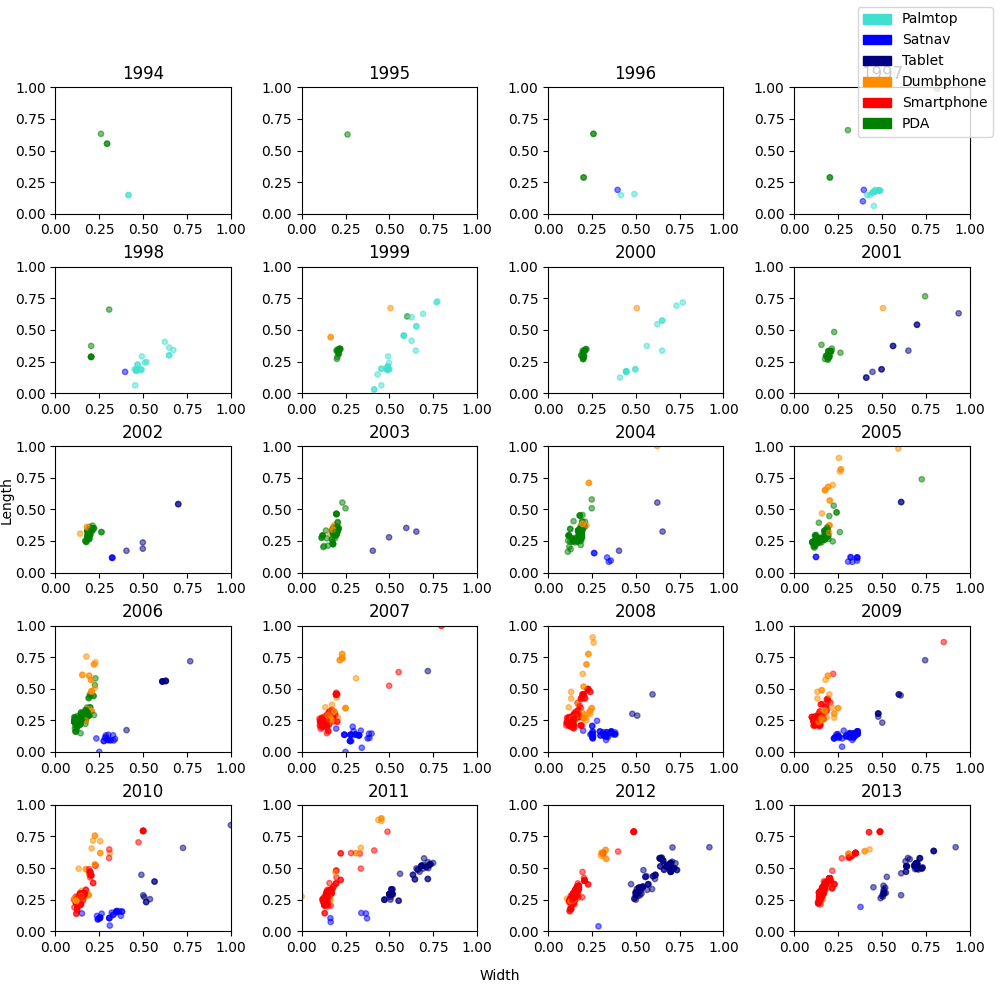
\includegraphics[width=0.5\textwidth]{../Visualisations/B/length-width-ctype-syear.png}
    \caption{Length against width of each mobile device from 1994 to 2013,
	coloured by the estimated device type. The length and width are
	normalised between 0 and 1.}
    \label{fig:DimensionsYear}
\end{figure}

Similarly, Figure \ref{fig:AspectRatioYear} plots each device's display
aspect ratio and overall aspect ratio over time with subplots for each release
year.
Once again, the devices are colour by their estimated type to assist in visual analysis.

%Show the time segment plots - aspect ratios
\begin{figure}
    \centering
    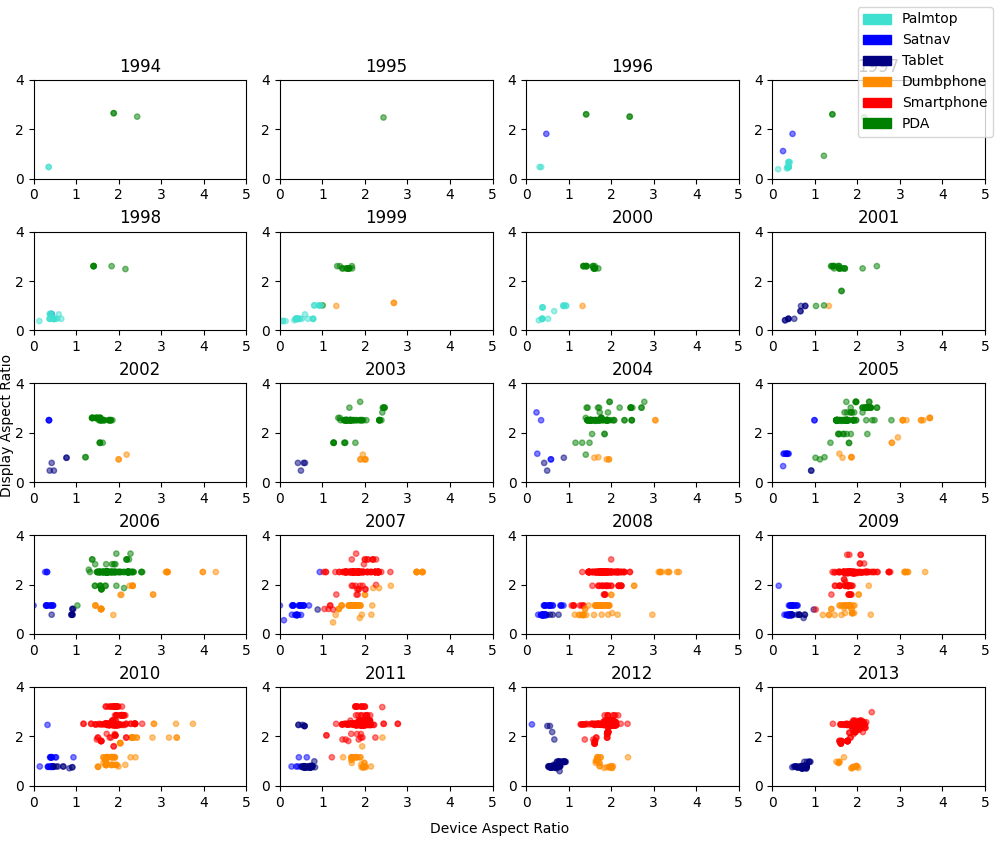
\includegraphics[width=0.5\textwidth]{../Visualisations/B/dr-r-ctype-syear.png}
    \caption{Device aspect ratio against display aspect ratio of each mobile
	device from 1994 to 2013, coloured by the estimated device type.}
    \label{fig:AspectRatioYear}
\end{figure}

%Figure \ref{fig:DimensionsYear} is a time series plot for each devices width against its length. Figure \ref{fig:AspectRatioYear} plots each devices aspect ratio against its corresponding display aspect ratio. Each device is present in exactly one of the plots from the years 1994-2013. Once again, the devices are colour coded to assist in visual analysis.

Finally, Figure \ref{fig:MarketShareYear} shows the year to year market share
between 1989 and 2013 of each device type as a percentage (top) and as a count
(bottom). Each share is coloured by its device type as before. This allows
one to compare the growth of different types over time and to gauge the popularity of the market between years.

%Figure \ref{fig:MarketShareYear} however is slightly different. In this stackplot, each device is plotted by its percentage market share over the years.

%Show the combined market share plot
\begin{figure}
    \centering
    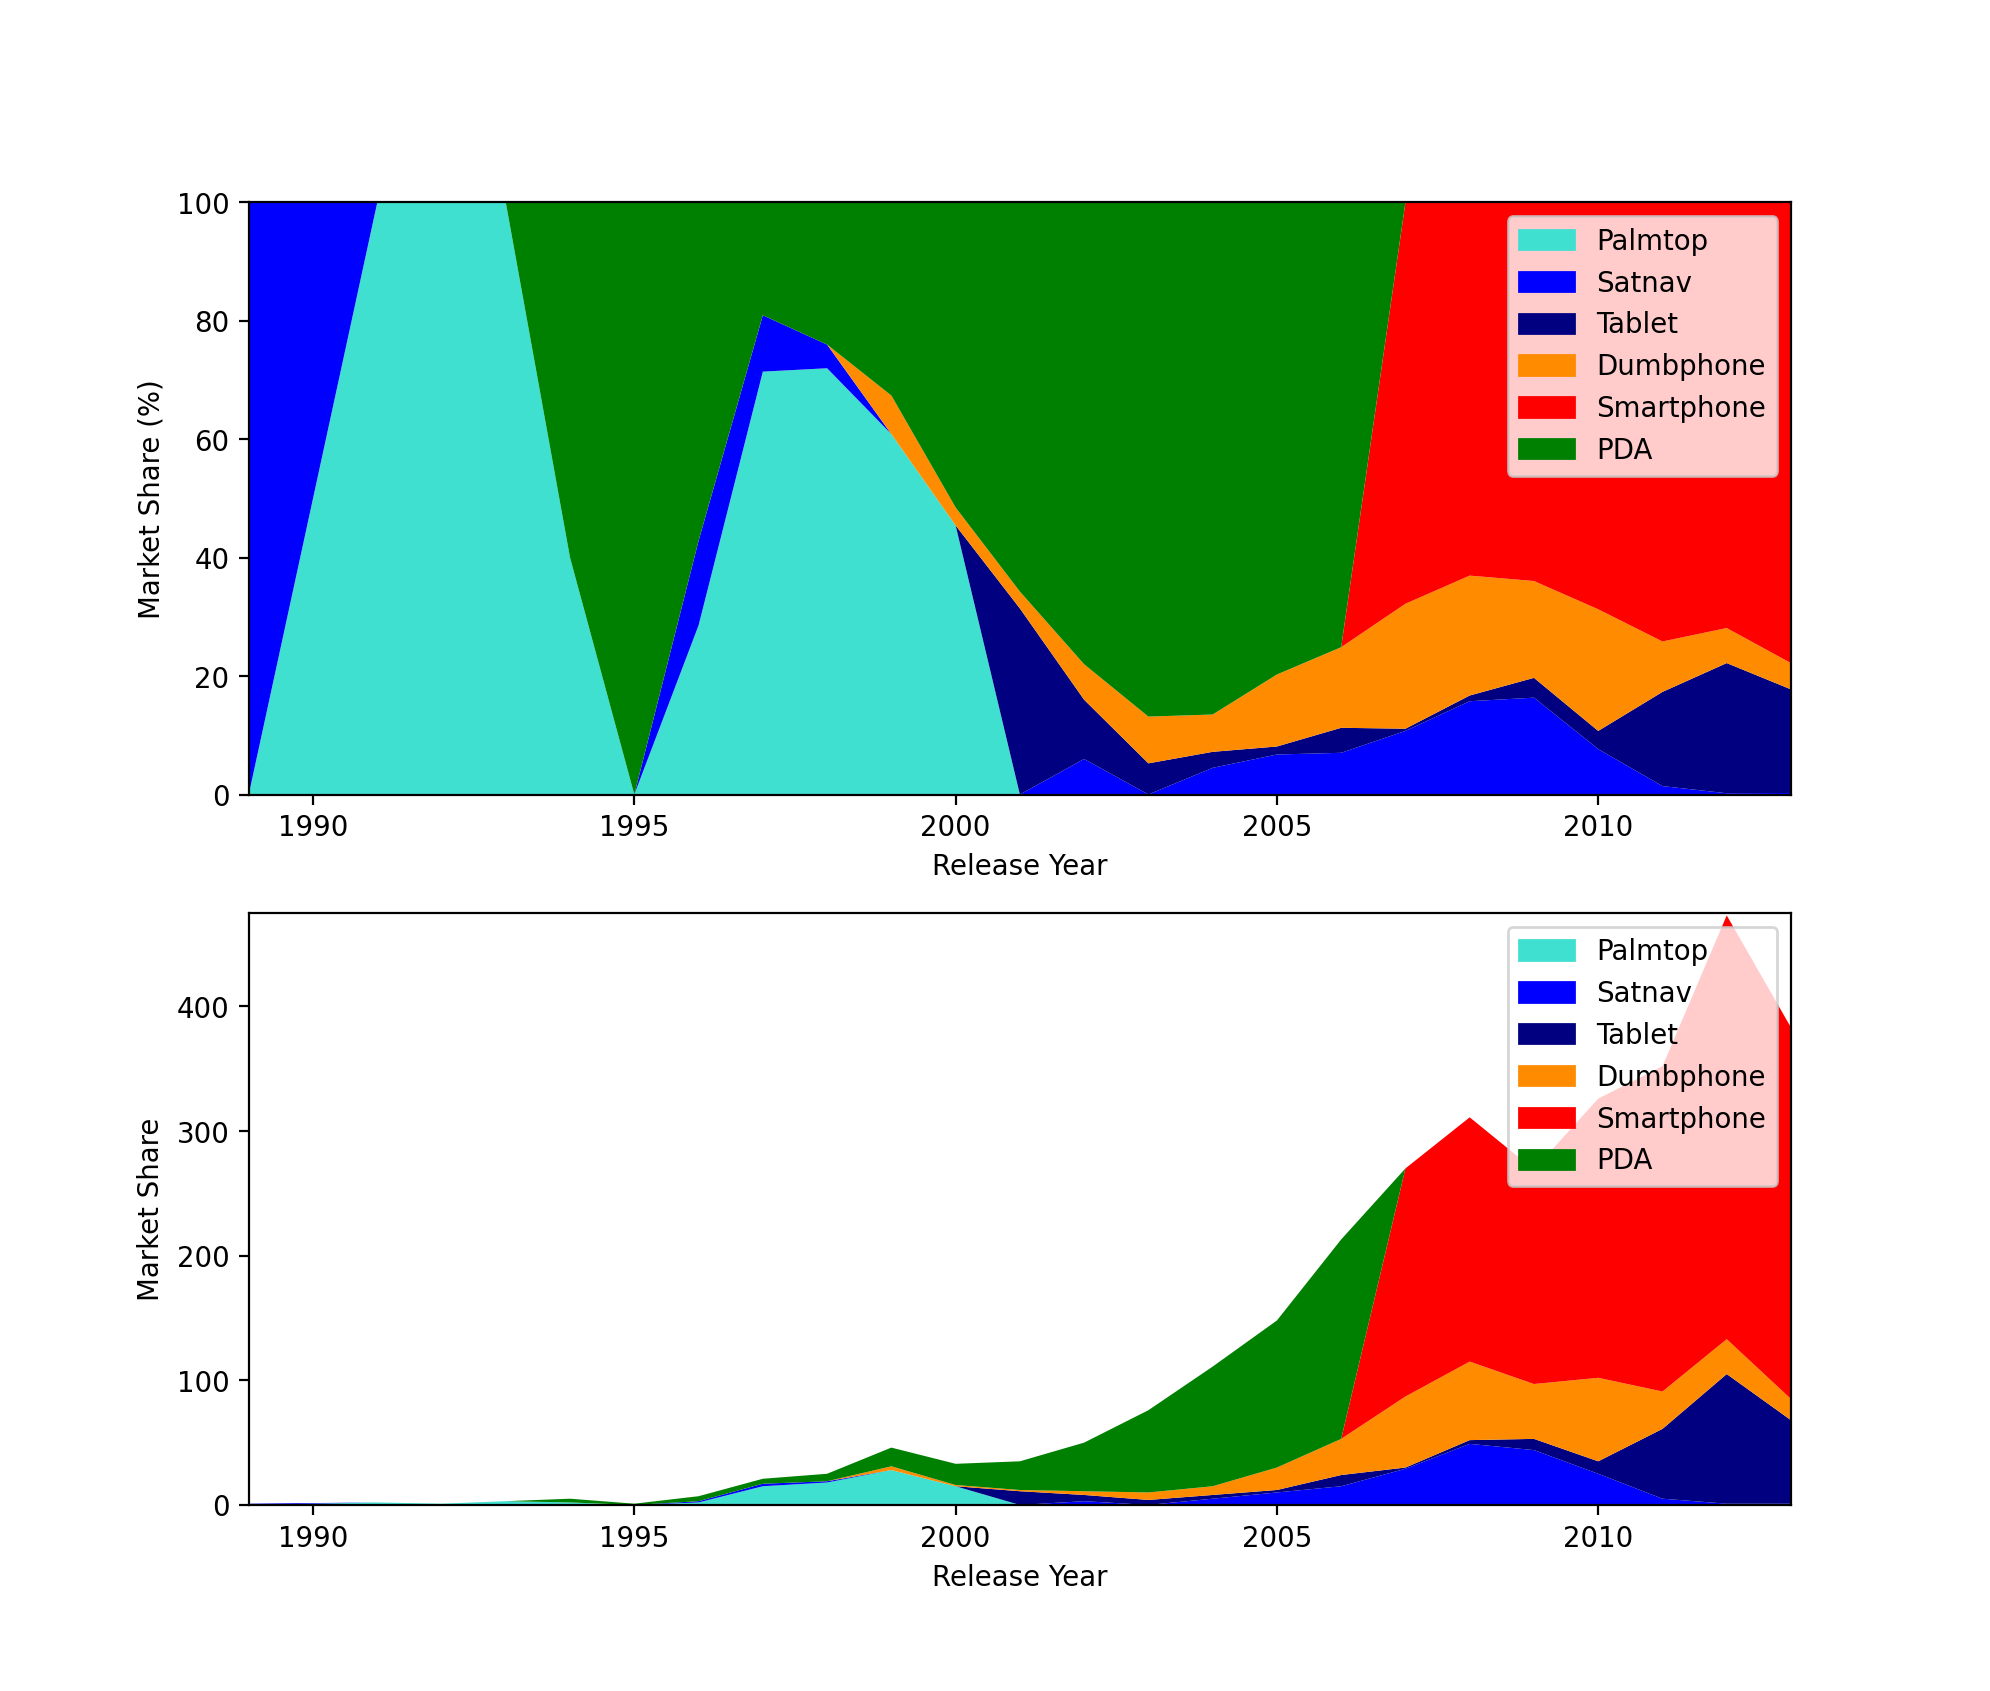
\includegraphics[width=0.5\textwidth]{../Visualisations/B/share-year.png}
    \caption{The market share of each device type from 1989 to 2013,
	coloured by device type. The percentage of the yearly market is shown
	in the top figure and the all time market share is shown in the
	bottom figure.}
    \label{fig:MarketShareYear}
\end{figure}

\subsection{Design Evaluation}
%Explain how your interactive visualisation has been evaluated and what sort of changes/modifications were applied to derive your final interactive visualisation.

As before, the visualisations were evaluated based on utility, comprehension
and insightfulness.

Figures \ref{fig:DimensionsYear} and \ref{fig:AspectRatioYear} were
originally plotted over all years from 1989 to 2013, however years 1989 to 1993
did not contribute to many insights as few devices were released over that
period in the data. For this reason a visually appealing five by four array of
subplots arranged in chronological order from left to right and top to bottom
made the most sense in terms of utility and insightfulness. Furthermore,
Figure \ref{fig:DimensionsYear} was based on Figure \ref{fig:HeightvsWidth} in
Section \ref{sec:A}, and so gained from previous evaluation discussed above.

%The time segment plots were both based on their single predecessors. However, they were expanded to show the progression through time.

Figure \ref{fig:MarketShareYear} was initially only the bottom plot, which
made it difficult to draw insights of trends prior to 2000. This is due to the
huge growth in the mobile device market which occured over the turn of the
century. As a result, the relative percentages were added as context and
displayed in top plot alongside the absolute market share plot.

%The market share plot was created to give a more absolute understanding of the numerical shift in market share trends.
%The market share plot was initially based on the absolute numbers, but was very difficult to interpret before 2005 due to the increase in the mobile market over the 2000s. It was shifted to relative to make the market share more obvious, and the absolute one was attached below to provide more information for comparison.

\subsection{Justifications}
%Why certain axes arrangement(s) was(were) used and how they would help to see the information you would need to see,
%Why certain visual variables were used and how they would help to see the information you would need to see,
%Why certain interaction was used and how that would assist analytic processes.

Figure \ref{fig:DimensionsYear}
was based on its single predecessor (Figure \ref{fig:HeightvsWidth}), with the
same information and axes arrangement.
However, it was expanded alongside
Figure \ref{fig:AspectRatioYear}
to show the progression through time. They were split into 20 different
subplots in five by four matrices, arranged left-to-right and top-to-bottom for ease of
understanding. This allowed for the evolution of the clusters to be observed
through time, and to make it obvious when a cluster was superseded or shifted in
the market. This also could be animated, but this makes it more difficult to
compare across longer spans of time.

Figure \ref{fig:MarketShareYear}
was arranged with the proportion of market share on the $y$-axis, and the release year on the $x$-axis.
It makes most sense to place time on the $x$-axis since we typically read
information from left to right.
%since the horizontal axis should be the one assigned to the evolution through time.
An area plot was selected instead of a line plot, as recommended in the lectures,
since it is filled and thus displays the market share proportions more naturally.
The colours were matched with those selected in earlier plots, to ensure visual continuity and ease of understanding.
The two plots were stacked together with their time axes aligned -- allowing for easy comparison of the absolute and proportional times for each year.

\section{Future Predictions}
%If you were to predict or anticipate a newly emerging mobile device type, what sort of evidence(s) you can visually show to easily detect such emergence? For instance, if you only had access to the data between 1989 and 2010, how would you anticipate new types which became dominant during 2011 and 2013 without seeing the data corresponding to 2011 – 2013?
The final question asks us to find evidence that could predict or anticipate an emerging category of mobile devices.
Two methods were used to answer this question. One was to predict possible future emerging mobile device categories by directly observing the market share graph with each type of mobile device. The other was to identify additional metrics to predict possible emerging mobile device categories by observing changes in these metrics.

In particular, assuming we only have data from 1989 to 2010, our goal is to predict the new type of mobile devices that became dominant from 2011 to 2013.
We begin by discussing the market share plot.
As we can see from Figure \ref{fig:market-2010}, smartphones started to appear in 2007 and have grown rapidly in market share every year since then. Tablets started to appear in 2009, but only occupy a small market share. PDAs, on the other hand, have seen a steady decline in market share. It is therefore reasonable to assume that after 2010, smartphones will continue to grow steadily and replace PDAs as the dominant type of mobile device.

Now we move on to the second method. Consider the metric $m$ given by
\[ m = \frac{\text{pixel density}}{\text{depth}}. \]

The reason for choosing this metric is that smartphones generally have a higher pixel density than other categories of mobile devices, while their depth is generally less than other categories of mobile devices. Therefore, the metric is able to differentiate smartphones from other categories of mobile devices.

By looking at the line graph in Figure \ref{fig:pixel}, it can be seen that from 2008--2010, the average pixel density/depth is increasing linearly, which means that the pixels of mobile devices are increasing and their thickness is decreasing during the decade, thus we can deduce that the reason for this result is the mass production of cell phones, especially in 2006-2010, when the slope is gradually increasing. Thus, we can predict that the proportion of cell phones in the market share will increase significantly in the next 3 years. Comparing the market share graphs, we can see that cell phones did dominate the market share from 2008 to 2013, thus confirming our prediction.

\begin{figure}
    \centering
    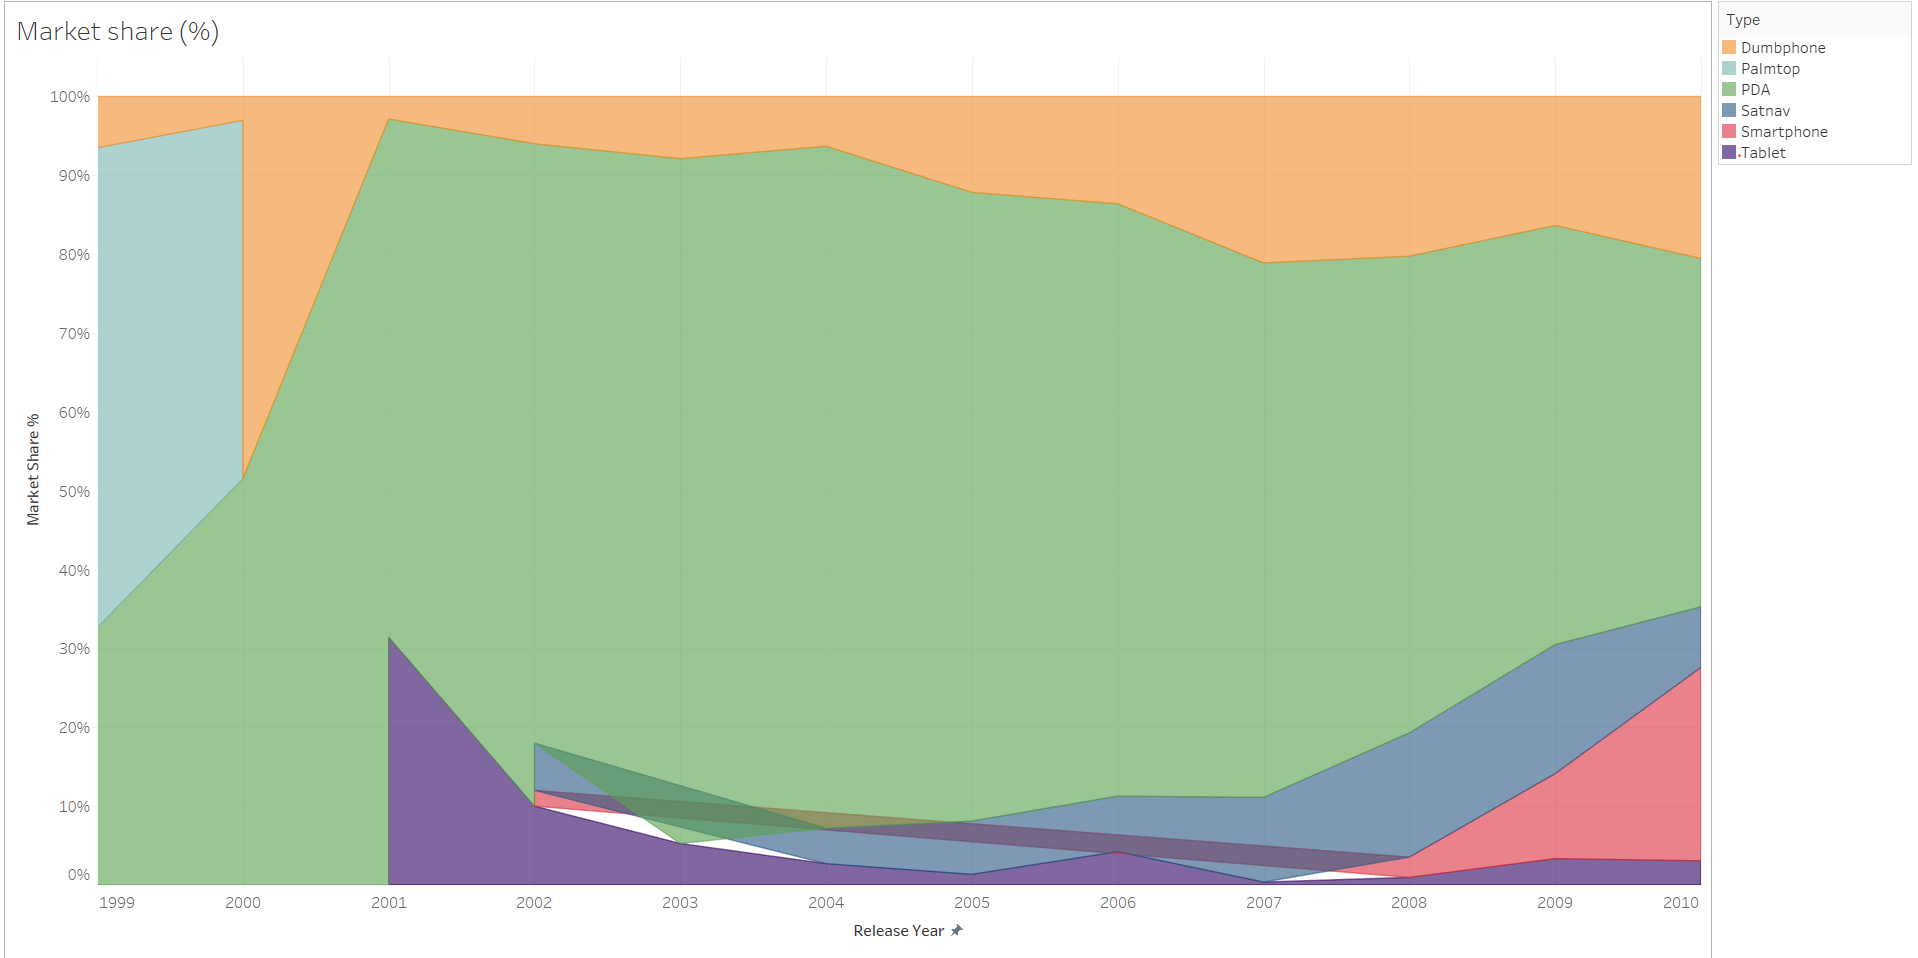
\includegraphics[width=0.5\textwidth]{Market Share.PNG}
    \caption{An interactive visualisation of the percentage market share of each
	mobile device type from 1999 to 2010, coloured by type.}
    \label{fig:market-2010}
\end{figure}

\begin{figure}
    \centering
    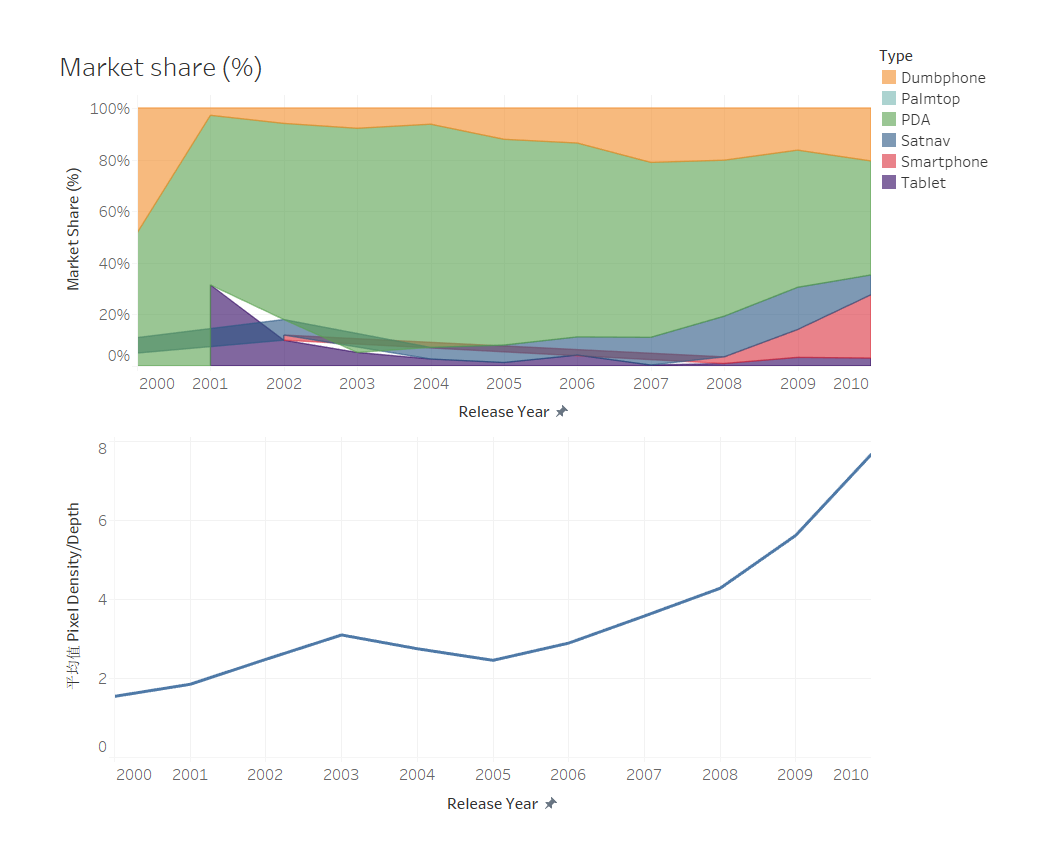
\includegraphics[width=0.5\textwidth]{Piexel density.png}
    \caption{An interactive visualisation of the market share percentage
	area plot (top) and the average $m$ metric (bottom) over time.}
    \label{fig:pixel}
\end{figure}

%Interactive Visualization (or multiple visualizations) allows you to “see” the pieces of information that lead to the answers to the above three questions 1-A/B/C.

\subsection{Visualisation}
Figure \ref{fig:market-2010} is an area chart with each device plotted by its percentage market share over the years from 1999 until 2010, which is the time interval we can currently observe. Each device has been assigned a unique color. From the color area, it can be seen that it is the market share of mobile devices in different years. Thus, the share of mobile devices in different categories for each year and how the share of different mobile devices has changed over time can be easily visualized.

Figure \ref{fig:pixel} is a composite plot consisting of two subplots. One is an area chart of the market share of different types of mobile devices across years just like Figure \ref{fig:market-2010}, the other one is a line graph that shows a linear trend of the average pixel density/ width ratio of devices versus the year of mobile device release. The line graph shows this relationship more clearly, enhances the visualisation, and aids the user to make further predictions.

\subsection{Design Evaluation}
%Explain how your interactive visualisation has been evaluated and what sort of changes/modifications were applied to derive your final interactive visualisation.
The market share plot in Figure \ref{fig:market-2010} was created here to observe the evolution of the share of different categories of mobile devices and thus to extrapolate the conclusions we wanted to draw that which is the possible emerging type of mobile devices in the future.

For Figure \ref{fig:pixel}, the market share plot was used to show the actual market share situation and could be compared with our prediction results to verify whether our guess is correct. The line graph is used to show the trend of the average Pixel density/depth to predict the future market share change.

\subsection{Justifications}
%Why certain axes arrangement(s) was(were) used and how they would help to see the information you would need to see,
%Why certain visual variables were used and how they would help to see the information you would need to see,
%Why certain interaction was used and how that would assist analytic processes.
Figure \ref{fig:market-2010} shows a chart of the proportional market share of the different categories of mobile devices. This visual chart arranges the proportion of market share vertically and the year of release horizontally, as the horizontal axis is supposed to be assigned to an evolving axis. And as before, we used an area plot rather than a line plot. This is because the area plot is filled and it could show a proportion of the market share of mobile devices in different categories and how they are changing more clearly. 

For Figure \ref{fig:pixel}, the market share plot is arranged vertically in proportion to the market share and horizontally in the year of release of the mobile device. This is because the horizontal axis should be assigned to the axis that evolves over time. And we also chose an area chart here. To ensure visual coherence and ease of understanding, the colors match those of the previously drawn graphs. The line graph is used to show the change of data over a continuous time interval or time span and is characterized by reflecting the trend of things changing over time or in ordered categories. The line graph clearly shows whether the data is increasing or decreasing, the rate of increase or decrease, the pattern of increase or decrease, and the peak characteristics. We use it to analyze the trend of data change over time, we use the horizontal axis in the line graph to represent the time span and the same time interval, and the vertical axis to represent the data values at different time moments.

\bibliography{bib}
\bibliographystyle{unsrt}

\end{document}
